\documentclass[11pt]{article}

\usepackage{amsmath}
\usepackage{graphicx}
\usepackage{multicol}
\usepackage{natbib}
\usepackage{wrapfig}
\usepackage{hyperref}
\usepackage{tabularx}
\usepackage{setspace}
\usepackage{comment}

\usepackage[compact]{titlesec}  
\titlespacing{\section}{0pt}{0pt}{0pt}
\titlespacing{\subsection}{0pt}{0pt}{0pt}
\titlespacing{\subsubsection}{0pt}{0pt}{0pt}

\oddsidemargin 0cm
\evensidemargin 0cm

\usepackage[margin=1in]{geometry}

\parindent 0cm
\parskip 0.5cm

\usepackage{fancyhdr}
\pagestyle{plain}
%\fancyhf{}
%\fancyhead[L]{AOSS Reference Sheet}
%\fancyhead[CH]{test}
\fancyfoot[C]{Page \thepage}

\newcommand{\vb}{\mathbf}
\newcommand{\diff}[2]{\frac{d #1}{d #2}}
\newcommand{\diffsq}[2]{\frac{d^2 #1}{{d #2}^2}}
\newcommand{\pdiff}[2]{\frac{\partial #1}{\partial #2}}
\newcommand{\pdiffsq}[2]{\frac{\partial^2 #1}{{\partial #2}^2}}
\newcommand{\topic}{\textbf}
\newcommand{\arcsinh}{\mathrm{arcsinh}}
\newcommand{\arccosh}{\mathrm{arccosh}}
\newcommand{\arctanh}{\mathrm{arctanh}}

\begin{document}

\appendix

\addtocounter{section}{3}
 
\section{Project Description}

\subsection{Background and Summary}

%The National Research Council has also acknowledged that ``climate models are continually moving toward higher resolutions via a number of different methods in order to provide improved simulations and more detailed spatial information'' \citep{NRC2012CLIMATEMODELS}.  

The next century is expected to see unprecedented changes to the climate system with extensive socioeconomic repercussions.  In the absence of an experimental test bed for global climate, global atmospheric modeling systems have been built to provide insight into potential future change in the climate system.  Although consensus has been reached on broad global changes that will occur, many outstanding questions remain on how regional or local climate will be affected in response to global change.  In particular, understanding extreme temperatures, precipitation and weather is key for informing local policymakers and communities, and informing the developing of adaptation policies.  However, restrictions on computational cost have inherently limited the finest resolution of our uniform-resolution global atmospheric models to 50-100 kilometers, far beyond the scale necessary for capturing many facets of regional climate.  Dynamically downscaled models which use global climate model data for boundary conditions are also known to suffer from spurious noise and do not provide two-way coupling between regional and global scales.  Consequently, there is a pressing need to develop a next generation of global atmospheric modeling systems that can properly address questions on these scales.

In response to the aforementioned need, the goal of this proposal is to develop a next-generation atmospheric modeling system that
\vspace{-0.4cm}
\begin{enumerate}
\item[(a)] is scalable (in both a strong and weak sense) on \textbf{massively parallel computers and hybrid architectures},
\item[(b)] remains valid on grid resolutions finer than 10km by solving the \textbf{non-hydrostatic global equations},
\item[(c)] supports \textbf{static and adaptive mesh refinement} to allow for proper communication between global an regional scales,
\item[(d)] addresses \textbf{known numerical issues with existing terrain-following coordinate models} at high horizontal resolutions, including horizontal pressure gradient errors and  and
\item[(e)] provides the \textbf{most accurate solution of the equations of motion} while limiting the need for artificial numerical diffusion. 
\end{enumerate}

\vspace{-0.4cm}
A key theme of this proposal will be \textbf{staggered nodal finite element methods (SNFEMs)}, which can be thought of as an optimal mixture of continuous and discontinuous nodal finite element methods (NFEMs).  These methods are described in detail in section \ref{sec:SNFEM}.  The central hypotheses of this proposal are as follows:

\vspace{-0.4cm}
\begin{itemize}
\item[(H1)] Horizontally staggered nodal finite element methods will provide an optimal or near-optimal treatment of wave motion, energy and enstrophy conservation and will reduce the need for significant artificial numerical diffusion compared to unstaggered methods.

\item[(H2)] Vertically staggered nodal finite element methods will improve the ability of the model to capture vertical stratification in the atmosphere, and improve the treatment of the pressure gradient force near rough topography.

\item[(H3)] A non-linear numerical diffusion operator based on either a variational multi-scale (VMS) or upwinding can be used to reduce diffusive errors in the finite element formulation over hyperviscosity, especially in the presence of steep gradients.
\end{itemize}

These hypotheses and proposal goals will be addressed via a structured set of research tasks:
\begin{itemize}
\item[(T1)] \textbf{Analyze the wave-like behavior} of the 1D and 2D SNFEMs and NFEMs under modified order-of-accuracy, prognostic variable staggering and choice of flux reconstruction function.

\item[(T2)] Implement 1D SNFEMs for \textbf{discretization of the vertical coordinate} in the Tempest framework (\S \ref{sec:TempestFramework}).  Analyze and contrast model results using the vertical SNFEM formulation.  Test sensitivity of horizontal pressure gradient errors to vertical order-of-accuracy and staggering.

\item[(T3)] Implement 1D SNFEMs for \textbf{discretization of the horizontal coordinate} in the Tempest framework.  Analyze and contrast model results for different choices of staggering, order-of-accuracy and viscous coefficients.

\item[(T4)] Develop and implement variational multi-scale (VMS) and upwind-type \textbf{dissipation mechanisms for both horizontal and vertical discretization}.  Analyze and compare simulation results.

\item[(T5)] Extend the Tempest framework to support \textbf{static and adaptive mesh refinement} with SNFEMs.
\end{itemize}

\vspace{-0.4cm}
The focus of this proposal on the development, analysis and implementation of new numerical methods fits well within the scope of NSF Computational Mathematics, which supports ``mathematical research in areas of science where computation plays a central and essential role, emphasizing design, analysis, and implementation of numerical methods and algorithms, and symbolic methods.''  A further strength of this proposal is its interdisciplinary character, bridging atmospheric science (represented by PI Ullrich) and mathematics (represented by co-PI Persson).  The numerical methods developed under this project will further have interdisciplinary application, and should be applicable to disciplines such as acoustics, aerospace, astrophysics and oceanography.

\subsection{Broader Impacts and Intellectual Merit} \label{sec:BroaderImpacts}

The goal of this project is to improve the state-of-the-art for global climate and weather forecasting models by improving the treatment of the underlying dynamics within these models and developing methods which are capable of being used at high horizontal resolutions.  This work has substantial societal consequences:
\vspace{-0.4cm}
\begin{itemize}
\item High-resolution and multi-resolution methods are directly applicable to regional scale climate problems: As mentioned above, changes in the behavior of mesoscale storm systems, pressure blocking events driven by topography (responsible for heat waves and cold spells), mountain snowpack, wildfires, topographically-driven precipitation, watershed-level hydrology, urban development and agriculture are all regional scale issues that are poorly addressed in current generation global climate modeling systems.
\item This technology is important for building global atmospheric models which are effective in regions of sharply varying topography, such as at the periphery of the California central valley.
\item The improved wave-capturing properties of these methods will have the potential to capture phenomena which are highly dependent on wave-like motion, such as the Madden-Julian Oscillation (MJO).
\item These advances have the potential to improve the technology that underlies meteorological models.  This particular framework can further be used for tropical cyclone forecasting by improving global resolution over the major global hurricane basins.
\item The multi-resolution framework can be used to test physical parameterizations in a multi-scale environment, to verify realistic performance of these parameterizations across scales.
\item The development of SNFEM for simulating the atmosphere could lead to their adoption in other fields, such as aerospace or computational biology.
\end{itemize}
\vspace{-0.4cm}
This project further seeks to improve the partnership between the National Center for Atmospheric Research (NCAR) and UC Davis by a mutual exchange of expertise on atmospheric dynamics.  Further, as a consequence of this work, a new next-generation numerical framework will be available for simulating atmospheric dynamics.  The PI intends to release this product (including all source code and documentation of implementation details) for use in future research as open source, and later integrate this work into the Community Earth System Model (CESM) \citep{JWHetal2013BAMS} for use in operational climate simulations.  The code for this project will be released under the Lesser GNU Public License (LGPL), which allows largely unrestricted access to the technology developed as part of this effort.  This project is further aimed at funding the thesis work of a graduate student through completion of their degree.

This project will further tie into the Dynamical Core Model Intercomparison Project (DCMIP), which is a major international effort that focuses on the components of atmospheric models that are responsible for solving the equations of motion.  The PI is currently a lead organizer of this effort.  DCMIP has previously run a two-week summer school and workshop in the summer of 2008 and 2012, with the next workshop planned for 2016.  These workshops have historically attracted over a dozen international modeling groups and over 30 graduate students to facilitate discussion of new numerical methods and provide an intensive educational experience for participants in global modeling.  The next workshop will specifically focus on developing numerical methods for simulating at high resolution, multi-resolution modeling and the coupling of model dynamics and physics.  It is expected that the graduate student and postdoc funded as part of this proposal will represent and showcase this work at the DCMIP workshop.

\subsection{Unique aspects of modeling the atmosphere}

The problem of simulating the general circulation of the atmosphere is unique in many ways.  First, the atmosphere itself only occupies a thin shell around the Earth of approximately $100\ \mbox{km}$ thickness, relative to the Earth's radius of $6371\ \mbox{km}$.  Second, although the atmosphere is largely uniform horizontally, it is strongly stratified in the vertical direction with pressures of $10^5\ \mbox{Pa}$ at the Earth's surface to $0.1\ \mbox{Pa}$ at the top of the stratosphere.  Third, the bottom of the domain is a rough unresolved boundary with local steepness that is strongly dependent on model resolution.  Fourth, unresolved physical processes on the sub-grid-scale, including condensation, vertical convection, turbulence and radiation, are essential for forcing the resolved-scale flow.

The atmospheric domain is typically discretized at a horizontal resolution of approximately $110\ \mbox{km}$ and a vertical resolution ranging from $100\ \mbox{m}$ in the lowest model levels to $3-4\ \mbox{km}$ near the model top.  The highest resolution uniform models that have been used for climate experiments are only at scales of $25\ \mbox{km}$, largely constrained by available computing power.  Variable-resolution modeling systems, which are capable of providing enhanced resolution over a particular regional patch, have recently been a subject of substantial interest and have pushed local climate resolution down to $10\ \mbox{km}$.  Nonetheless, even at these (relatively fine) horizontal resolutions, the horizontal-vertical aspect ratio is on the order of $\sim\ 100$.  Consequently, in accordance with the Courant-Friedrichs-Lewy (CFL) condition, explicit time stepping of the vertical operator would be a bottleneck on the maximum time-step size.  To overcome this difficulty, the hydrostatic approximation has been used to enforce instantaneous balance between the vertical pressure gradient force and gravity and so eliminates vertically propagating sound waves.  However, the hydrostatic approximation, which requires elimination of horizontal transport of vertical velocity, is no longer valid on scales below approximately $10\ \mbox{km}$ horizontally.  Since horizontal resolutions are quickly approaching this limit, the next generation of modeling systems will adopt the Navi\'er-Stokes equations in their unapproximated form.  To overcome the vertical CFL limitation, these systems have generally adopted an explicit temporal discretization in the horizontal in conjunction with an implicit temporal discretization in the vertical, also known as Horizontally Explicit Vertically Implicit (HEVI), coupled in the context of an Implicit-Explicit Runge-Kutta (IMEX-RK) framework \cite{}.

Atmospheric simulations are a benchmark application for exascale computing systems since many important climatological features are unresolved at current resolutions.  Consequently, any improvement to the simulation quality has the potential to significantly reduce computational expense.

\subsection{Topography and the pressure gradient problem}

Model topography is typically introduced by transforming the vertical coordinate so that the Earth becomes a coordinate surface \cite{}.  Compared with alternatives, such as cut cells, immersed boundary methods or embedded boundary methods, this approach is simple and easily retains the accuracy of the underlying discretization.  However, this approach also has one key disadvantage:  specifically, a straightforward implementation of terrain-following coordinates leads to a non-orthogonal coordinate frame that has the effect of polluting the relative homogenous horizontal pressure and density fields with strong vertical gradients associated with vertical stratification.  Errors are particularly pronounced near regions with the strongest underlying topography.

Since the sharpest gradients in topography are typically adjacent to local peaks, an increase in horizontal resolution is expected to lead to steeper slopes.  A simple example of this problem is depicted in Figure \ref{fig:MountainSlopeResolution}, where an isolated Utah mountain is plotted with a variable horizontal resolution.  As the horizontal mesh is refined, the maximum slope also increases in steepness to $32^\circ$ at the finest resolution.  Under a HEVI discretization, an initially balanced flow over such a mountain will only remain balanced if the pressure gradient terms on the left-hand-side of the horizontal momentum equations (\ref{eq:NonhydroEqn1})-(\ref{eq:NonhydroEqn2}) (those treated via an explicit method) and those on the right-hand-side (treated with an implicit method) cancel each other exactly.  However, a low-order discretization and coupling strategy between the horizontal and vertical discrete pressure gradient terms (that is, standard dimensional splitting) is insufficient to maintain balance.  Figure \ref{fig:SpuriousMountainNoise} shows the vertical velocity in the presence of rapidly varying bottom topography, and highlights the effects of inaccurate evaluation of the horizontal pressure gradient term for models with a terrain-following coordinate.  Since typical vertical velocities for large-scale weather systems are $\sim 0.01\ \mbox{m\ s}^{-1}$, these perturbations represent an error of nearly $50\%$.

The issue of the pressure gradient problem has significant implications for global atmospheric modeling, with efforts to tackle this problem stretching back as far as the late 1970s \citep{ZIJ1977BzPdA, DTMZIJ1986MAP}.  As global models reach to finer spatial scales, the pressure gradient problem leads to an increasingly polluted dynamical solution near steep topography.  The typical solution to this problem is easily considered crude:  A diffusive filter is repeatedly applied to topography data until the maximum slope fits within a specified tolerance and there is no sign of numerical noise associated with steep topography.  This approach has the obvious consequence of severely damaging the quality of the solution near topography, and leading to an effective grid resolution much coarser than the grid would allow.  Topographically driven precipitation, which is particularly important for estimating mountain snow-pack, is weakened substantially under this approach.  Further, atmospheric pressure blocking, which is responsible for stationary pressure systems and the development of heat waves / cold spells, is suppressed under topographical smoothing.  Other approaches which address mitigation of this problem include the use of cut-cells \citep{JSSHPAD2013GMDD}, coordinate surface smoothing \citep{JBK2011MWR}, reconstruction of pressure along horizontal coordinate surfaces \cite{GZ2012MWR}, or formulations which preserve consistency with the continuous operator \citep{SJL1997QJRMS}.  In the context of high-order FEM, this proposal advocates removing errors by improving the accuracy of the coupling between the horizontal and vertical discrete pressure gradient operators.

\begin{figure}
\begin{center}
\includegraphics[width=4in]{MountainSlopeResolution.png}
\end{center}
\caption{The averaged slope of topography increases monotonically with increased horizontal resolution.  Here an image of an isolated Utah mountain is shown with variable horizontal resolution.  Image courtesy of Dr. Tina Chow, UC Berkeley.} \label{fig:MountainSlopeResolution}
\end{figure}

\begin{figure}
\begin{center}
\includegraphics[width=3in]{SpuriousMountainNoise.png}
\end{center}
\caption{Vertical velocity for a balanced flow over a rapidly varying mountain range.  Because of inaccurate evaluation of the horizontal pressure gradient term, models with terrain-following coordinates can generate significant spurious numerical errors in the presence of steep topography.  Here a hydrostatically balanced atmosphere initially at rest quickly generates a train of spurious internal mountain waves in response to numerical errors.} \label{fig:SpuriousMountainNoise}
\end{figure}

\subsection{The Tempest Framework} \label{sec:TempestFramework}

\begin{wrapfigure}{r}{2.5in}
\begin{center}
\includegraphics[width=2in]{A_CubedSphere}
\end{center}
\caption{The cubed-sphere grid.} \label{fig:CubedSphere}
\end{wrapfigure}

This proposal will use the Tempest framework as a starting point for research tasks T2-T5.  Tempest is a numerical atmospheric modeling framework (\url{https://github.com/paullric/tempestmodel}) \citep{PAU2014GMDa, PAU2014GMDb} implemented in C++ and MPI for solving partial differential equations in block-structured geometry.  The framework has been built by PI Ullrich to improve the ease of experimentation with numerical discretizations, particularly for applications in geophysical fluid dynamics.  The model currently supports a number of nodal finite-element methods including discontinuous Galerkin (DG) \cite{}, spectral element (SE) \cite{} and flux reconstruction (FR) \cite{}.  The large horizontal-vertical aspect ratio associated with the atmosphere requires a distinct treatment for horizontal and vertical operators; in order to preserve parallel scalability explicit time stepping is used for the horizontal discretization, whereas geometric stiffness associated with short spatial scales in the vertical require the use of an implicit operator.  Tempest implements a number of implicit-explicit (IMEX) time-stepping schemes to provide high-order coupling of the directional operators \citep{PAUCJ2012MWR}.  The equations of motion in the global model are based on a terrain-following height coordinate.  The model supports both limited-area (Cartesian) domains and global (spherical) domains, via the cubed-sphere grid (see Fig. \ref{fig:CubedSphere}).  Work is currently underway to integrate Tempest into the Community Earth System Model \citep{JWHetal2013BAMS} so the efforts from this proposal would be made available to the international modeling community.



%that uses a finite element discretization of the non-hydrostatic equations of motion.  It has been designed and built by the PI to improve the ease of experimenting with numerical discretizations in an Earth-system context.  It currently supports Discontinuous Galerkin (DG), Spectral Element (SE) and Flux Reconstruction (FR) \citep{HTH2007AIAA} methods using a horizontally-explicit vertically-implicit (HEVI) discretization, with coupling via Strang splitting \citep{PAUCJ2012MWR}.  The equations of motion are based on a terrain-following height coordinate and the simulation grid is either Cartesian or a cubed-sphere (Figure \ref{fig:CubedSphere}) \citep{PAUCJBVL2010JCP,PAUCJ2012JCP}.  The model is parallelized via MPI.  Figure \ref{fig:TempestBaroclinicInstability} shows the results at day 10 of the baroclinic wave test of \cite{PAUTMCJAS2013QJRMS} as simulated by the Tempest model.  It is eventually the goal that the Tempest model will be incorporated into the Community Earth System Model \citep{JWHetal2013BAMS}.  This proposal aims to use the Tempest framework as a foundation for software development and experimentation.

\begin{figure}
\begin{center}
\includegraphics[width=6in]{UMJSTest-Results}
\end{center}
\caption{A developing non-hydrostatic baroclinic instability simulated in the Tempest framework.  Relative vorticity shown.} \label{fig:TempestBaroclinicInstability}
\end{figure}

Traditional global atmospheric models use the hydrostatic approximation, which assumes that the vertical atmosphere is perpetually in a state of balance between pressure gradient and buoyancy forces.  In this case, vertical momentum is no longer tracked and is instead diagnosed from other state variables.  However, this approximation breaks down when the horizontal resolution is finer than roughly $10\ \mbox{km}$, and so the next-generation of global atmospheric models have instead turned to using the non-hydrostatic Euler equations (with shallow-atmosphere approximation):
\begin{align}
\label{eq:NonhydroEqn1} \pdiff{u^\alpha}{t} + u^i \nabla_i u^\alpha + \frac{1}{\rho} \left[g^{\alpha \alpha} \nabla_\alpha p + g^{\alpha \beta} \nabla_\beta p \right] + f (\vb{k} \times \vb{u})^\alpha &= - \frac{g^{\alpha \xi}}{\rho} \nabla_\xi p, \\
\label{eq:NonhydroEqn2} \pdiff{u^\beta}{t} + u^i \nabla_i u^\beta + \frac{1}{\rho} \left[g^{\alpha \alpha} \nabla_\alpha p + g^{\alpha \beta} \nabla_\beta p \right]  + f (\vb{k} \times \vb{u})^\beta &=  - \frac{g^{\beta \xi}}{\rho} \nabla_\xi p, \\
\label{eq:NonhydroEqn3} \pdiff{\theta}{t} + u^\alpha \pdiff{\theta}{\alpha} + u^\beta \pdiff{\theta}{\beta} &= - u^\xi \pdiff{\theta}{\xi}, \\
\label{eq:NonhydroEqn4} \pdiff{u^\xi}{t} + u^\alpha \nabla_\alpha u^\xi + u^\beta \nabla_\beta u^\xi + u^\xi \nabla_\xi u^\xi &= - \frac{1}{\rho} \nabla^\xi p - g_c, \\
\label{eq:NonhydroEqn5} \pdiff{\rho}{t} + \frac{1}{J} \pdiff{}{\alpha} (J \rho u^\alpha) + \frac{1}{J} \pdiff{}{\beta} (J \rho u^\beta) &= - \frac{1}{J} \pdiff{}{\xi} (J \rho u^\xi).
\end{align}  Here $\alpha$ and $\beta$ are arbitrary horizontal coordinates with basis vectors $\vb{i}$ and $\vb{j}$, $\xi$ is a vertical coordinate with unit basis vector $\vb{k}$, the index $i$ spans each coordinate, $g^{ij}$ denotes the contravariant metric, $J = \sqrt{\det g_{ij}}$ is the metric Jacobian, $\nabla_i$ denotes the covariant derivative along the $i^{th}$ coordinate, $g_c$ is gravity, $f$ is the Coriolis parameter, $\rho$ is the density, $\vb{u} = u^\alpha \vb{i} + u^\beta \vb{j} + u^\xi \vb{k}$ is the vector velocity and $\theta$ is the potential temperature.  Einstein summation notation is used for repeated indices.  These equations are closed via the equation of state
\begin{equation*}
p = p_0 \left( \frac{R_d (\rho \theta)}{p_0} \right)^{c_p / c_v},
\end{equation*} where $R_d$ is the ideal gas constant, $p_0$ is a reference pressure and $c_p$ and $c_v$ denote the specific heat capacity of dry air at constant pressure and constant volume.  Observe that (\ref{eq:NonhydroEqn1})-(\ref{eq:NonhydroEqn4}) are given in a non-conservative form; this formulation is generally desirable over the conservative formulation (where momentum and $\rho \theta$ are prognostic variables) since this form can more readily conserve quantities relevant to atmospheric motion, such as angular momentum and potential enstrophy, and (depending on the discretization) can lead to a more accurate treatment of wave-like motions \citep{JTTJW2005JCP}.

This equation set has been studied in detail for over a century, and a wide range of mature numerical methods are now available for modeling its solutions.  Finite element methods (FEM), which include both the spectral element (SE) method and the discontinuous Galerkin (DG) method, have a long history in the field of computational fluid dynamics stretching back to the 1970s (see \cite{patera:84,maday:89,FBSR1997JCP,BCCWS1998JCP}).  Recent advances in FEM motived by \cite{HTH2007AIAA} also no longer impose the need for a conservative equation set when formulated with a DG discretization.  However, FEM have only recently been adopted by the atmospheric modeling community \citep{taylor:97,FXGJSHTW2002JCP,FXGTER2004MWR,AFMTJT2004MWR,NTL2005MWR,FXGMR2008JCP,JFKFXG2012JCP}.  The primary motivation for the adoption of FEM in global atmospheric codes has been the need for methods which perform well on very large-scale parallel systems (those with hundreds of thousands to millions of computing cores).  To its advantage, FEM can provide near-optimal scalability on parallel computing systems with minimal bandwidth requirements (that is, it minimizes the message size needed to convey information between neighboring elements) and so, unlike many global spectral and semi-Lagrangian methods, are tenable for use on these systems.  The need for scalable numerical methods is essential with the rapid expansion of massively-parallel supercomputers in the past decade.  FEM can also be formulated to have many desirable mathematical properties, including mass and energy conservation, high-order accuracy, as well as discrete preservation of the adjoint and annihilator properties of the gradient, divergence and curl operators.  Further, recent work on FEM has led to techniques for effective positivity and monotonicity filtering \citep{OGMATASC2013}.  Consequently, the Community Atmosphere Model (CAM), for the first time, has adopted the spectral element method of \cite{MTAF2010JCP} as the default dynamical core.  Many other modeling groups are now working on adopting finite element methods as the basis for their dynamical cores, including the NUMA model of \cite{JFKFXG2012JCP}.  FEM are also likely candidates for adoption on the U.K. Met Office dynamical core and the upcoming model from the Korean Institute of Atmospheric Prediction Systems (KIAPS).

\subsection{Staggered Nodal Finite Element Methods} \label{sec:SNFEM}

\begin{figure}
\begin{center}
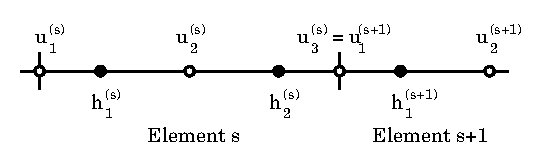
\includegraphics[width=4in]{SEStaggered}
\end{center}
\caption{An example 3rd order horizontal staggering of 1D velocity (u) and height (h) state variables for a SE/DG SNFEM for the shallow water equations.  Here $u$ nodes are placed at Gauss-Lobatto quadrature points and $h$ nodes are placed at Gaussian quadrature points.  The superscript denotes the element number and the subscript denotes the sub-grid-scale index.} \label{fig:SEStaggered}
\end{figure}

\begin{figure}
\begin{center}
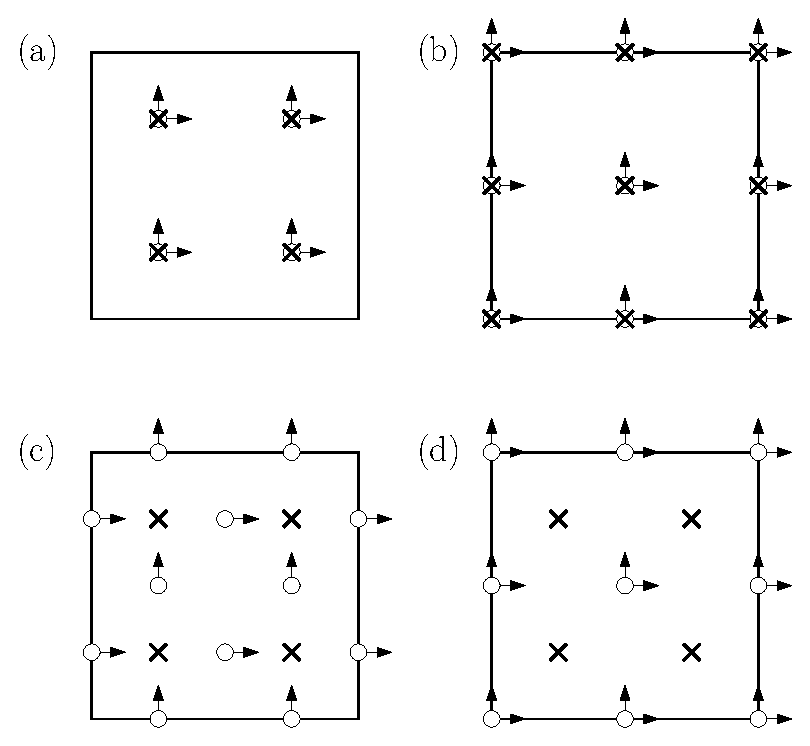
\includegraphics[width=3in]{NodalArrangement}
\end{center}
\caption{Four options for the placement of scalar ($\times$) and velocity variables (arrows): (a) nodal discontinuous Galerkin, (b) nodal Spectral Element, (c) C-grid SNFEM, (d) B-grid SNFEM.} \label{fig:NodalArrangement}
\end{figure}

In the past year there has been growing interest in the atmospheric modeling community in the use of staggered nodal finite element methods (SNFEM).  In the context of nodal FEM, SNFEM represent a class of methods where scalar (density, pressure, potential temperature) and velocity variables are stored at different nodal points within an element.  One such example of a 3rd order 1D hybrid SE/DG method is depicted in Figure \ref{fig:SEStaggered}.  Four possible arrangements of prognostic variables are depicted in Figure \ref{fig:NodalArrangement} for a 2D SNFEM.  Closely related to SNFEMs are mixed finite element methods, which have been used for elliptic problems since the 1970s by \cite{PRJT1977MAFEM}.  SNFEMs are particularly desirable since they generalize the staggered grid approach which has been a staple of atmospheric models since the work of \cite{AAVRL1977GCM}.  Staggered grid models are the standard in the ocean modeling community, and have been the foundation for many current and previous generation atmospheric models.  Staggered grids are used in the CAM finite-volume dynamical core \citep{SJL2004MWR}, the previous default dynamical core in CAM, and its successor the Geophysical Fluid Dynamics Laboratory (GFDL) finite-volume cubed-sphere model \citep{WMPSJL2009NMSPF}.  They have also been adopted in the Weather Research and Forecasting (WRF) model \citep{SWCKJBDJetal2001}, which is the standard in regional weather forecasting, and its spiritual successor the global Method for Prediction Across Scales (MPAS) model \citep{WCSJBKMGDLDFSHPTDR2012MWR}.

This proposal uses a differential formulation of SNFEM, where the differential operators on Gauss-Legendre (GL) and Gauss-Lobatto-Legendre (GLL) nodes (that is, those typically associated with nodal DG and SE discretizations, respectively) arise naturally from the flux reconstruction methods of \cite{HTH2007AIAA}.  This method can be applied in conjunction with the direct stiffness summation operation (which averages co-located state values on GLL nodes) when continuity is desired.  An operator for stabilization / diffusion, which is necessary for the application of these methods to long-term climate simulations, will be developed based on the work of \cite{OGMNLJROMATPAU2013}.  It is well-known that an optimal choice of grid staggering can greatly improve the treatment of atmospheric waves \citep{DAR1994MWR}, but it is not immediately clear how staggering of variables should be handled in the context of FEM.  However, recent efforts by \cite{DBLG2009CS} and \cite{CJCJS2012JCP} have investigated a standard low-order 1D SNFEM staggering and generally found that SNFEM retain the desirable properties of FEM (parallel scalability, mass/energy conservation and a discrete analogue of the gradient, divergence and curl operators).  Further, when the staggering is chosen correctly, these methods also retain the beneficial properties of staggered grid methods.  The PI has also investigated the ability of several standard numerical methods to properly capture the diffusive and dispersive properties of the 1D linear wave equation, and the results suggest that SNFEM greatly outperforms competing methods (see Table \ref{tab:ShortestResolvedWave} and \cite{PAU2013QJRMS}).

\begin{table}
\begin{center}
\begin{tabular}{ccc}
\hline & \multicolumn{2}{c}{\underline{Shortest Resolved Wave}} \\
Method & Order 3 & Order 4 \\
\hline \hline Finite Volume & $12.53\ \Delta x$ & $9.98\ \Delta x$ \\
Spectral Volume & $11.94\ \Delta x$ & $9.16\ \Delta x$ \\
Discontinuous Galerkin & $10.01\ \Delta x$ & $7.87\ \Delta x$ \\
Spectral Element & $8.33\ \Delta x$ & $8.87\ \Delta x$ \\
SNFEM & $6.68\ \Delta x$ & $5.56\ \Delta x$ \\
\hline
\end{tabular}
\end{center}
\caption{Shortest wavelength which is resolved to at least 0.5\% error in both the diffusive and dispersive error components, obtained from analysis of the 1D linear wave equation, for several methods of third- and fourth-order accuracy.} \label{tab:ShortestResolvedWave}
\end{table}

\subsection{Justification of Hypotheses}

\textbf{Why are these hypotheses justified?  Why are we using SNFEMs?}

- Contrast the non-hydrostatic equation set versus traditional approaches using the hydrostatic equations

\begin{figure}
\begin{center}
\includegraphics[width=5in]{CAMSEScalability.png}
\end{center}
\caption{Simulated year per day of three atmospheric dynamical cores at 28km global resolution on Intrepid (IBM BG/P), including the global spectral model (EUL), regular latitude-longitude finite-volume model (FV) and the hydrostatic spectral element model (SE) when run in conjunction with 28km land model and 11km sea ice and data ocean.  Near perfect scalability is observed for the spectral element model down to one element per core (86400 cores).  Reproduced from \cite{JDJEKJEONGetal2011IJHPCA}.}
\end{figure}


The hypotheses of this proposal has been formulated based on past success of massively parallel finite element methods (FEMs) \citep{JDJEKJEONGetal2011IJHPCA}, the analysis of staggered methods performed by \cite{JTTJW2005JCP}, an understanding of the wave-like properties of numerical methods built from \cite{PAUCJ2011JCP}, the analysis of low-order SNFEM performed by \cite{CJCJS2012JCP} and preliminary analysis of SNFEM discussed in section \ref{sec:SNFEM}.  In addition to the central hypothesis stated above, we further hypothesize the following: 
\vspace{-0.4cm}
\begin{enumerate}
\item The C-grid SNFEM (see section \ref{sec:SNFEM}) with exact mass matrix will provide optimal wave-like behavior, but the method with inexact mass matrix will be more computationally efficient.

\item A high-order vertical discretization combined with a high-order horizontal-vertical coupler will greatly reduce errors associated with the pressure gradient problem.

\item Overall SNFEM will reduce errors in the atmospheric dynamical core (the component of atmospheric models responsible for solving the equations of fluid motion), particularly for phenomena with relatively short spatial scales.
\end{enumerate}
\vspace{-0.4cm}
The remainder of this proposal is as follows:  Broader impacts and intellectual merit are described in section \ref{sec:BroaderImpacts}.  The Tempest model, which will be the foundation for software development as part of this proposal, is described in section \ref{sec:TempestModel}.  The pressure gradient problem is explained in detail in section \ref{sec:PressureGradientProblem}.  SNFEMs are described in section \ref{sec:SNFEM}.  The proposed research project is found in section \ref{sec:Research} and the research plan and timeline in section \ref{sec:ResearchPlan}.  Future work is described in section \ref{sec:FutureWork}.

\subsection{Detail of the Proposed Research} \label{sec:Research}

The overarching theme of this research is the development of a next-generation multi-resolution non-hydrostatic atmospheric modeling environment based on (optimal) FEM/SNFEM which addresses known issues in pushing atmospheric models to high resolutions.  This work will also address the horizontal pressure gradient problem, which is a notorious issue in atmospheric models in the vicinity of steep topography.

There is clear utility to the geophysics community in the adoption of new and improved numerical methods, and SNFEM has the potential to greatly enhance the capability of current atmospheric dynamical cores to accurately and efficiently simulate the atmospheric equations of motion.  This research will be addressed in four parts, corresponding to the four objectives of the proposal:
\begin{itemize}
\item[(a)] Implementation and analysis of 1D and 2D arbitrary-order SNFEM (\S \ref{sec:AnalysisSNFEM}),
\item[(b)] Implementation and analysis of a SNFEM vertical discretization (\S \ref{sec:VerticalSNFEM}),
\item[(c)] Implementation and analysis of high-order coupling strategies using implicit-explicit Runge-Kutta methods (\S \ref{sec:CouplingSNFEM})
\item[(d)] Implementation and analysis of a SNFEM horizontal discretization in the context of block-based mesh refinement (\S \ref{sec:HorizontalSNFEM})
\end{itemize}  Each of these items can be pursued independently, and each is expected to be the basis for one or two future publications.  This research is expected to be carried out over a period of three years.

\subsubsection{Analysis of 1D and 2D staggered nodal finite element Methods} \label{sec:AnalysisSNFEM}

\begin{figure}
\begin{center}
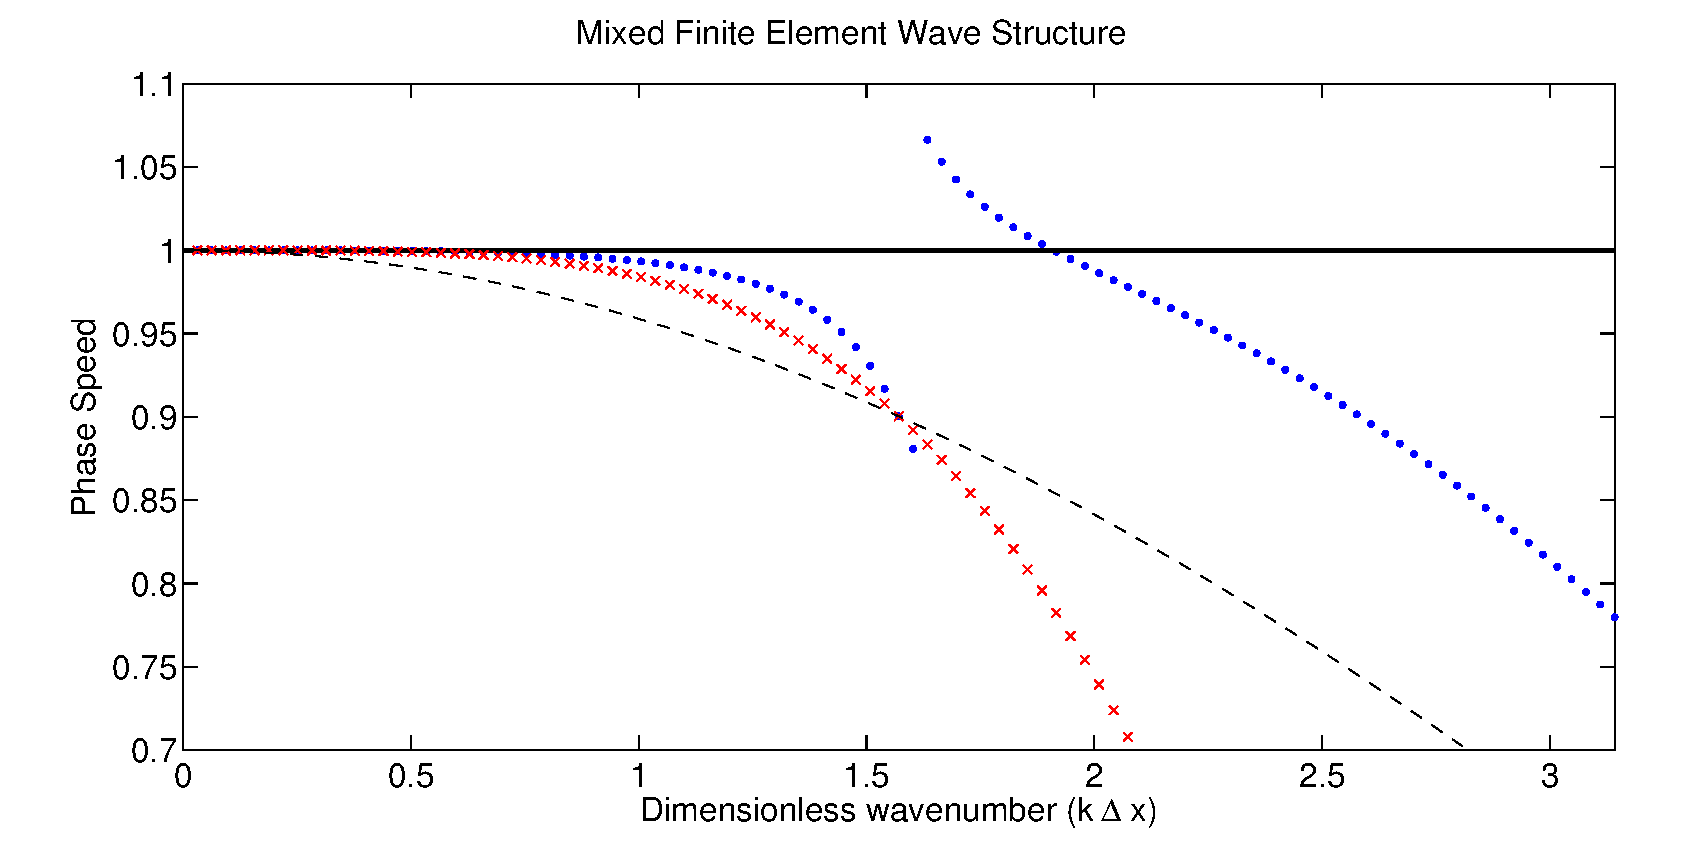
\includegraphics[width=5in]{HFEM_ThirdOrder}
\end{center}
\caption{A dispersion analysis of the right-going mode of the 1D third-order staggered nodal finite element method depicting normalized phase speed as a function of dimensionless wavenumber.  The solid line denotes the exact phase speed, normalized to $1$.  The dotted blue curve depicts the SNFEM phase speed, the dashed line depicts the phase speed of a standard staggered second-order scheme and the red crosses ($\times$) depict the phase speed of the third-order SE method.  Note that since the SE method is unstaggered, the phase speed must go to zero at $k \Delta x = \pi$.  Both SNFEM and SE have the same number of degrees of freedom per element, but SNFEM boasts the best long-wavelength ($k < \pi/2$) and short-wavelength ($k > \pi/2$) properties.  The presence of the spectral gap at $k \Delta x = \pi / 2$ will be addressed in this work.} \label{fig:SNFEMEigenstructure}
\end{figure}

To a close approximation, the atmosphere is in a state of geostrophic and hydrostatic balance.  The dynamic character of the atmosphere is governed by a slow adjustment process which gives rise to wave motion over all scales.  Accurate treatment of these waves is important to capture departures from geostrophic balance, and to ensure that the adjustment process is correct and free from spurious numerical errors.  As shown by \cite{PHLCJMATRDN2010JAMES}, an accurate treatment of the equations of motion is also important to avoid errors due to grid imprinting.  The capability of a numerical method to capture wave-like motion in atmospheric models is typically evaluated using dispersion analysis.  This mathematical technique decomposes the discrete response in the atmospheric model into diffusive and dispersive errors introduced by the discretization.  Diffusive errors are typically associated with an unphysical loss of wave energy from the system and dispersive errors are associated with unphysical ringing, corresponding to an incorrect treatment of individual wave speeds.  A key paper by \cite{DAR1994MWR} used dispersion analysis to demonstrate the superior performance of staggered grids for modeling geophysical flows.  More recently, \cite{MAHAW2009SIAMJNA} (and later \cite{TMASJT2012QJRMS}) applied dispersion analysis to the SE method in the context of geophysical motions.  They found that, although the SE method possessed good long-wave characteristics, the unstaggered nature of the scheme led to a short-wavelength regime with unphysical backwards energy propagation.  There is currently no thorough analysis of SNFEM for use in atmospheric models.  Preliminary results shown in Figure \ref{fig:SNFEMEigenstructure} suggest that the SNFEM method possesses superior wave properties for the 1D wave equation, with the exception of a small gap at wavenumber $\pi / 2$.  A thorough dispersion analysis of this method, extending preliminary work to 2D geophysical problems, would be incredibly beneficial for determining any outlying issues with the formulation of the method prior to its use in atmospheric modeling.  Further, this analysis would provide guidance in choosing a SNFEM formulation that preserves desirable geophysical properties, including geostrophic balance on the $f$-plane.  A thorough analysis must address several outstanding questions:

\begin{figure}
\begin{center}
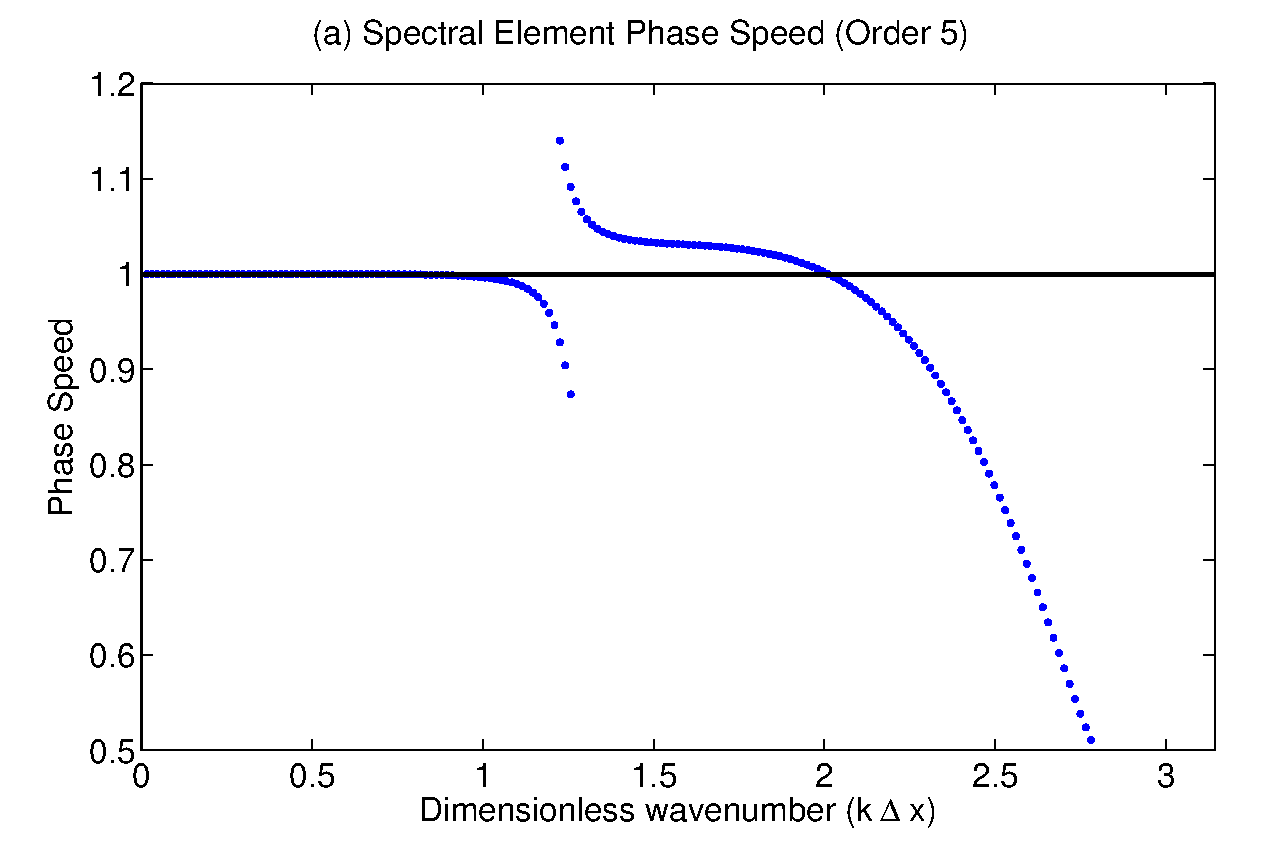
\includegraphics[width=3.2in]{SE_UnmodifiedDispersion}
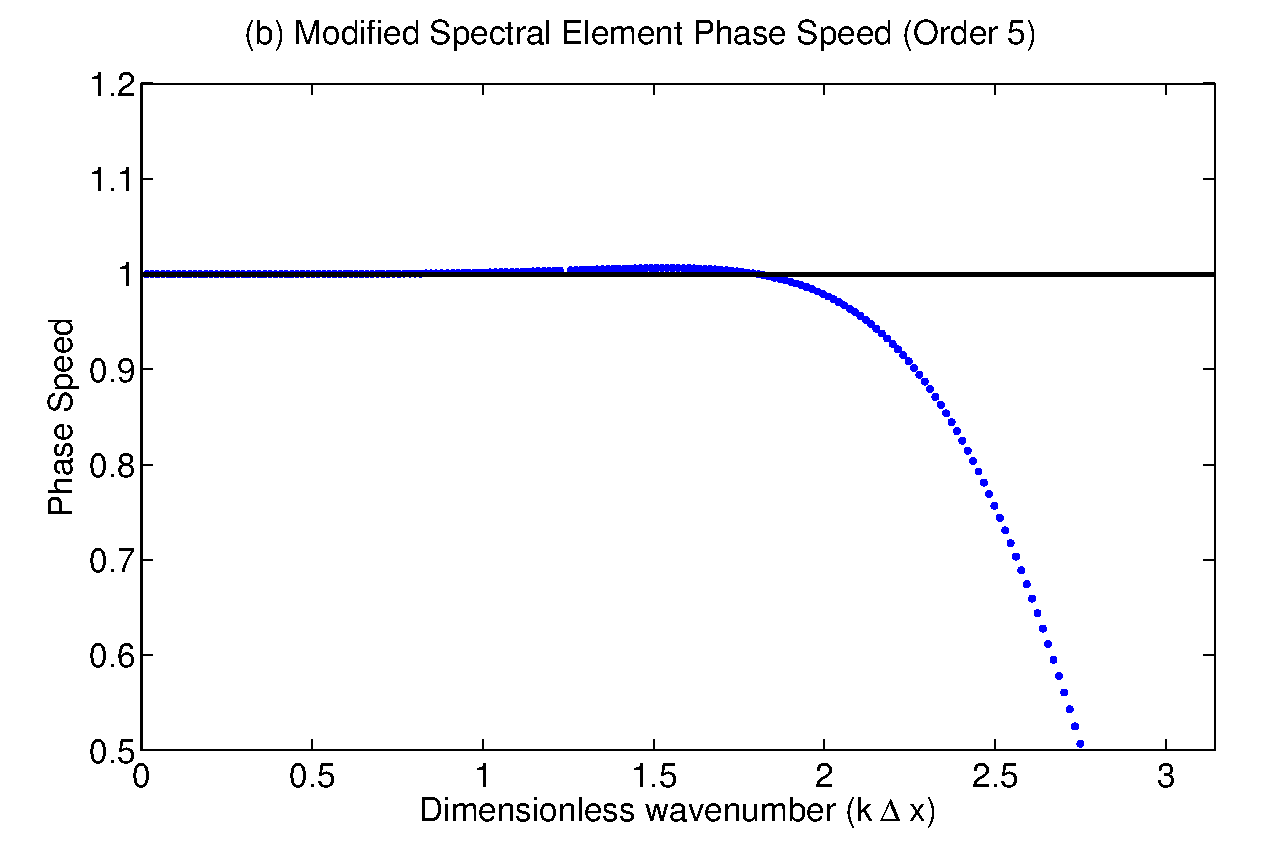
\includegraphics[width=3.2in]{SE_ModifiedDispersion}
\end{center}
\caption{(a) Dispersion relation for the unmodified SE method of order 5 showing a spectral gap and (b) Dispersion relation for the SE method using a modified basis where the spectral gap has been removed.  The solid line depicts the exact phase speed.} \label{fig:SEMDispersionGap}
\end{figure}

\begin{itemize}
\item The ``spectral gap'' is a phenomenon that often appears when a numerical method adopts a non-uniform grid to simulate the linear wave equation.  It is associated with an unphysical jump in the phase speed (see Figure \ref{fig:SNFEMEigenstructure}) which can lead to inaccurate treatment of certain wave numbers.  This gap can be fixed by either partial mass lumping \citep{ASMTCC2012QJRMS}, the application of dissipation (such as upwinding, as in the discontinuous Galerkin approach), or by an improved choice of the functional space within an element (modified basis method).  The modified basis method has been verified by the PI to successfully remove the spectral gap for the SE method and improve the accuracy of the method (see Figure \ref{fig:SEMDispersionGap} and \cite{PAU2013QJRMS}).  This project aims to study how the choice of dissipative operator and basis functions affects the spectra of the SNFEM approach, and if the spectral gap can be eliminated for the linear 1D and 2D shallow-water equations using a similar approach.  It is hypothesized that the spectral gap can be completely eliminated at all orders-of-accuracy through a combination of judiciously chosen dissipative operator and/or an improved choice of basis functions.

\item An extension of the SNFEM analysis to 2D is important to understand the behavior of SNFEM in a context which is relevant to geophysical motions.  In particular, this project is interested in an extension of the 1D analysis to the 2D linear shallow-water equations with non-zero Coriolis parameter $f$.  It is not currently understood if high-order SNFEM will share similar dispersion properties to the staggered finite-difference schemes which were analyzed by \cite{DAR1994MWR}.  Further, it is known that the arrangement of nodal points can have a significant effect on the dispersive properties of the underlying method.  Consequently, this effort aims to compare and contrast the different arrangements of nodal points (see Figure \ref{fig:NodalArrangement}) and their influence on the wave-capturing properties of the underlying SNFEM.  It is hypothesized that the C-grid arrangement of Figure \ref{fig:NodalArrangement}c will produce an optimal dispersion relationship.

\item Another issue that requires investigation is the behavior of SNFEM at refinement boundaries.  Atmospheric models that support variable resolution are becoming increasingly important in addressing issues related to extreme weather and regional climate change \citep{WCSJBKMGDLDFSHPTDR2012MWR}.  However, as pointed out by \cite{PAUCJ2011JCP}, in the presence of grid refinement staggered grid methods cannot distinguish between incident waves and artificially reflected waves.  As a consequence, energy in the incident mode tends to be reflected at grid refinement interfaces, leading to potential contamination of the solution in a region of enhanced resolution.  To further understand this behavior, an analysis of SNFEM in the presence of grid refinement is needed.
\end{itemize}

\subsubsection{A SNFEM Vertical Coordinate} \label{sec:VerticalSNFEM}

There has recently been renewed interest in improving the treatment of the vertical discretization in global atmospheric models.  The accurate representation of vertical wave modes is essential for models of the atmosphere, especially for those with wavelengths near the grid scale, where numerical errors typically appear.  Traditionally the vertical coordinate for the non-hydrostatic fluid equations has either been discretized in the Eulerian frame via a second-order Charney-Phillips \citep{JGCNAP1953JAS} or Lorenz grid \citep{AASM1988JAS}, or via a semi-Lagrangian approach such as \cite{SJL2004MWR}.  However, little work has been performed to develop high-order vertical coordinates due to a number of outstanding issues.  First, higher-order generalizations must somehow deal with the no-flux boundary conditions at the model bottom and top without loss of accuracy, especially near the surface where accurate treatment of dynamics is paramount.  Second, as observed by \cite{JTTJW2005JCP}, \cite{JT2006QJRMS} and \cite{MDTRDA2007JCP} the choice of vertical coordinate (whether height-based, mass-based or entropy-based) implies an optimal vertical staggering of prognostic variables for maintaining correct behavior for wave motions relevant to the atmosphere.  Third, unstaggered discretizations (that is, discretizations where all prognostic variables are stored on model levels) possess stationary computational modes which can potentially damage the numerical solution and can degrade the quality of the solution.  As in the horizontal direction, unstaggered FEM leads to waves with zero phase speed in the limit as wavelength $\lambda \to 2 \Delta x$ (see Figure \ref{fig:SNFEMEigenstructure}).  Unlike the horizontal, these wave modes can be dramatically enhanced by an implicit treatment of the vertical at high Courant number.

This proposal will develop, analyze and implement the SNFEM machinery for use as an arbitrary-order vertical discretization for the non-conservative formulation of the fluid equations, isolating terms which are relevant to vertical motion (from the right-hand-side of (\ref{eq:NonhydroEqn1})-(\ref{eq:NonhydroEqn5})).  The SNFEM prognostic variable staggerings can be easily composed in differential form using interpolation and differentiation operators built in accordance with the DG and SE discretizations that arise from the FR method (see Table \ref{tab:StaggeringOperators}).  The use of SNFEM is natural for vertical discretizations:  No-flux boundary conditions are natural in the context of FEM, and the structure of individual elements (that is, the tendency for nodal values to be concentrated near element edges) lends itself readily to improved resolution in the atmospheric boundary layer.  Further, SNFEM inherits the mimetic properties of SE methods and so the vertical operator will automatically conserve both mass and discrete energy.

The analysis component of this proposal will generalize and extend the work of \cite{JTTJW2005JCP} to understand how acoustic, inertia-gravity waves and the Rossby wave modes respond to different staggerings of prognostic variables, locations of interior nodes, choice of FR reconstruction function and order-of-accuracy in the context of SNFEM.  In total, of the prognostic variables $\rho$, $u$, $v$, $w$ and $\theta$ and the diagnosed mass flux $\mathcal{F}_\rho = \rho w$ and Exner pressure $\Pi$, there are $2^5$ different options for staggering on model levels and interfaces (assuming $\rho$, $u$ and $v$ are kept together).  Of these options only a limited subset exhibit optimal wave-propagation properties and are free of stationary computational modes.

%This proposal aims to generalize and extend the work of \cite{JTTJW2005JCP} to understand how acoustic, inertia-gravity waves and the Rossby wave modes respond to different staggerings of prognostic variables, locations of interior nodes and order-of-accuracy in the context of SNFEM.  

%Other staggering options may be explored in conjunction with the effect of a variable order-of-accuracy.  In addition the following questions will be addressed:

\begin{table}
\caption{Composition of interpolation $\mathcal{I}$ and differentiation $\mathcal{D}$ operators for several choices of staggering.  Subscript $e$ denotes variables defined on interfaces (Gauss-Lobatto-Legendre nodes) and $n$ represents variables defined on model levels (Gauss-Lobatto nodes).  For operator $\mathcal{I}$ and $\mathcal{D}$, the subscript denotes the target ($e$ or $n$) and the superscript denotes the origin.  In accordance with \cite{JT2006QJRMS}, the pressure gradient in the vertical is reformulated as $\rho^{-1} \nabla p = \theta \nabla \Pi$, where $\Pi$ is the Exner pressure ($\Pi_n(\rho, \theta) = c_p \left[ R_d \rho \theta / p_0 \right]^{R_d/c_v}$).} \label{tab:StaggeringOperators}

\begin{center}
\begin{tabular}{cc|ccc}
\hline  & & \multicolumn{3}{c}{\underline{Choice of Staggering}} \\
Variable & Operator & DG $(\rho_n \theta_n u^\xi_n)$ & SNFEM-L $(\rho_n \theta_n, u^\xi_e)$ & SNFEM-CP $(\rho_n, u^\xi_e \theta_e)$ \\
\hline \hline $\displaystyle \Pi_n$ & & $\Pi_n(\rho_n, \theta_n)$ & $\Pi_n(\rho_n, \theta_n)$ & $\Pi_n(\rho_n, \mathcal{I}_n^e \theta_e)$ \\[2.5ex]
$\theta$ & $\displaystyle u^\xi \pdiff{\theta}{\xi}$ & $(u^\xi_n) \mathcal{D}_n^n \theta_n$ & $(\mathcal{I}_n^e u^\xi_e) (\mathcal{D}_n^n \theta)$ & $(u^\xi_e) (\mathcal{D}_e^e \theta_e)$ \\[2.5ex]
$u^\xi$ & $\displaystyle \theta \pdiff{\Pi}{\xi}$ & $\theta_n \mathcal{D}^n_n \Pi_n$ & $(\mathcal{I}_n^e \theta_n) (\mathcal{D}^n_e \Pi_n)$ & $\theta_e (\mathcal{D}^n_e \Pi_n)$ \\[2.5ex]
$\rho$ & $\displaystyle \frac{1}{J} \pdiff{}{\xi} (J \rho u^\xi)$ & $\displaystyle \frac{1}{J_n} \mathcal{D}^n_n (J_n \rho_n u^\xi_n)$ & $\displaystyle \frac{1}{J_n} \mathcal{D}^e_n \left[ J_e (\mathcal{I}_e^n \rho_n) u^\xi_e \right]$ & $\displaystyle \frac{1}{J_n} \mathcal{D}^e_n \left[ J_e (\mathcal{I}_e^n \rho_n) u^\xi_e \right]$ \\[2.5ex]
\hline
\end{tabular}
\end{center}
\end{table}

%\begin{itemize}
%\item How do acoustic, inertia-gravity waves and the Rossby wave modes respond to different staggerings of prognostic variables, locations of interior nodes and order-of-accuracy?  This work aims to generalize and extend the work of \cite{JTTJW2005JCP}, who answered this question for the set of second-order central discretizations with arbitrary prognostic variable staggering.  The accurate representation of atmospheric wave modes is essential for models of the atmosphere, especially for the wave modes with the shortest wavelength, where numerical errors typically appear.

%\item What is the optimal approach for solving the implicit system that arises from the vertical discretization?  The matrix system that arises in each column of the model under a SNFEM discretization has a block-tridiagonal structure with a dominant off-diagonal.  This work intends to determine which approach leads to the most efficient solution of the implicit system.  The options for solvers include Jacobian-free Newton-Krylov (JFNK)-type methods, stabilized bi-conjugate gradient methods or a Jacobian construction / direct solver (with or without Schur complement).  Further, this proposal is interested in whether a Rosenbrock approach (that is, only computing a linearly implicit solution to the matrix system such as in \cite{PAUCJ2012MWR}) can be used in place of a fully implicit solution. 
%\end{itemize}

\subsubsection{Improved Horizontal-Vertical Coupling} \label{sec:CouplingSNFEM}

This research will investigate one approach for obtaining uniform high-order accuracy in both time and space by using a novel strategy for combining the horizontal, vertical and temporal discretization.  The time discretization must account for the treatment of horizontal motions by an explicit discretization and vertical motions by an implicit discretization; a technique known as horizontally explicit vertically implicit (HEVI).  Second-order and higher one-step methods are usually referred to as Implicit-Explicit Runge-Kutta (IMEX-RK) methods, and many such methods have been proposed in the literature \citep{UASJRRJS1997AMM, CACMHK2003ANM}.  Recently, recognizing that high-order coupling is necessary for next-generation non-hydrostatic atmospheric models, many of these methods have been analyzed in the context of HEVI discretizations by \cite{HWSJLNW2013JCP}.

This proposal targets an issue that has not been addressed in the atmospheric science literature:  Namely, can a high-order IMEX-RK method in conjunction with a high-order vertical discretization reduce errors associated with the pressure-gradient problem? (see the description of the pressure gradient problem in section \ref{sec:PressureGradientProblem})  The Tempest model will be used as a testbed for this study, in conjunction with either high-order FEM or SNFEM.  Different IMEX-RK methods will be investigated, implemented and compared in terms of accuracy and efficiency in order to determine which coupler leads to the lowest pressure gradient errors, and whether the associated cost makes this approach worthwhile.

\subsubsection{SNFEMs and Block-Based Mesh Refinement} \label{sec:HorizontalSNFEM}

SNFEMs show great promise in their application to geophysical problems.  Given a new numerical method, the development of an operational dynamical core is typically performed in three stages:  First, a global shallow water model is developed to verify that the method performs well for problems with 2D fluid characteristics similar to those of the global atmosphere.  Second, a 3D regional Cartesian-geometry climate model is developed to ensure that the method can perform well with a large horizontal-vertical aspect ratio.  Third, the vertical treatment from the Cartesian model is incorporated into the shallow-water model to produce an operational 3D dynamical core.  Tempest (see section \ref{sec:TempestModel}), which supports both Cartesian and cubed-sphere geometry, will be used as a framework for SNFEM development, and will greatly ease the development at each of these stages.

The adoption of mesh refinement in the global atmospheric modeling community is fairly recent, although a number of major modeling centers are currently pushing this capability to operational general circulation models \citep{WCSJBKMGDLDFSHPTDR2012MWR, LMHSJL2013MWR, CMZCJMAT2013MWR}.  The Tempest model uses an implementation of mesh refinement based on the block-adaptive strategy of \cite{MJBPC1989JCP}, with development in collaboration with the Chombo research group at LBNL \citep{ChomboDesign}.  Since only density and tracers will be conserved (which are discretized with the DG operators), an implementation of SNFEM in the block-based mesh refinement framework will be a fairly straightforward modification of the existing methodology.

Once dynamical core development is complete, verification must be performed to ensure consistency with analytical test cases, and intercomparison with other dynamical cores.  The standard test case suite in the shallow-water regime was established by \cite{WDHJS1992JCP}.  More recently, a test case suite for 3D atmospheric dynamical cores has been proposed as part of the Dynamical Core Model Intercomparison Project (DCMIP), documented in \cite{DCMIP2012TESTCASES}.  These test suites further provide the opportunity for intercomparison of the SNFEM dynamical core with other operational dynamical cores via DCMIP and other scientific publications.  Once verification is complete, future efforts will tackle the addition of moisture and physical parameterizations to the dynamical core.

This project will benefit greatly from the PI's past experience in atmospheric model development as author of the MCore high-order finite-volume modeling environment (see, for instance, \cite{PAUCJBVL2010JCP,PAUCJ2012MWR,PAUCJ2012JCP}).  The end goal of this work will be to develop a fully functional open-source dynamical core which is available for general research use by the atmospheric modeling community.

\subsection{Research Plan} \label{sec:ResearchPlan}

This project seeks funding for one postdoctoral researcher for two years and one graduate student researcher for three years.  Over the course of their employment, the postdoctoral researcher will work with the PI on the implementation of the SNFEM framework using the Tempest codebase, development of test problems and additional assistance with analysis of the SNFEM.  Simultaneously, the graduate student researcher will be in charge of the 1D and 2D analysis of SNFEM, with 2D analysis carrying over into the second year.  In the second year, the graduate student researcher will work to test out the various permutations of SNFEM and study the role of the vertical discretization and coupling mechanism on model accuracy in the presence of steep topography.  Finally, in their third year, the graduate student researcher will be responsible for validation and verification of the 3D SNFEM framework code, including applications to idealized scenarios in atmospheric dynamics.  The anticipated schedule for this project is given below:

\begin{tabularx}{\textwidth}{cX}
\hline
\textbf{Year 1} & $\cdot$ 1D analysis of arbitrary-order SNFEM, removal of spectral gap \\
& $\cdot$ 2D linear shallow-water analysis of arbitrary-order SNFEM \\
& $\cdot$ Implementation and testing of SNFEM vertical discretization \\
\hline
\textbf{Year 2} & $\cdot$ Continued analysis of 2D arbitrary-order SNFEM \\
& $\cdot$ Implementation and testing of SNFEM horizontal discretization \\
& $\cdot$ Validation / verification testing of global shallow-water SNFEM code \\
\hline
\textbf{Year 3} & $\cdot$ Analysis of arbitrary-order SNFEM in presence of grid refinement \\
& $\cdot$ Validation / verification testing of 3D Cartesian SNFEM code \\
& $\cdot$ Validation / verification testing of 3D global SNFEM code \\
& $\cdot$ Application of SNFEM framework to idealized atmospheric dynamics experiments \\
\hline
\end{tabularx}

We anticipate that at least five major peer-reviewed publications will arise from this work, including two covering the analysis of SNFEM (for each of the 1D and 2D formulation) and three covering the implementation of the SNFEM framework (for each of the vertical discretization, shallow-water model and 3D multi-resolution global model). Further, this work will be presented at major scientific meetings, including SIAM Geosciences, the meetings of the American Geophysical Union, the conference for Partial Differential Equations on the Sphere and the Dynamical Core Model Intercomparison Project 2016 Workshop and Summer School.

\subsection{Implications of the Proposal for Future Applications} \label{sec:FutureWork}

The work of this proposal has the potential to drive further innovations and form the basis for future research:

\begin{itemize}
\item The SNFEM framework that is produced from this work will be used to study dynamical relationships in the tropical atmosphere, following the work of \cite{JABAJM2005JAS,JABAJM2010CMS,JABAJM2012JAS}.  The highly accurate dispersion properties of this method will assist in testing asymptotic relationships governing wave interactions.

\item The SNFEM framework will be eventually coupled to a stochastic cloud model, following the work of \cite{BKYHJAB2005JAS,BMKJABAJM2010CMS} to study cloud-dynamics interactions and the viability of stochastic cloud models in a global modeling context.

\item The development of a global SNFEM ocean model will be pursued based on the work of this proposal.  This effort would be beneficial for several reasons:  Staggered grids are ubiquitous in the global ocean modeling community.  Consequently, the adoption of SNFEM for ocean modeling would be able to leverage existing technologies, while improving the spatial accuracy of existing methods.  This approach would also have similar near-optimal dispersive properties as SNFEM for the atmosphere.  This work could quickly lead to the use of a coupled atmosphere-ocean model based on SNFEM that would preserve numerical consistency between the atmosphere and ocean model component.
\end{itemize}

%\clearpage
%\bibliography{HybridFiniteElements}
\bibliographystyle{wileyqj}
{\setbox0\vbox{\bibliography{HybridFiniteElements}}}

\end{document}
